%% img/oracles/PolyHierarchy2.tex
%% Copyright 2019 Andrea Berlingieri
%
% This work may be distributed and/or modified under the
% conditions of the LaTeX Project Public License, either version 1.3
% of this license or (at your option) any later version.
% The latest version of this license is in
%   http://www.latex-project.org/lppl.txt
% and version 1.3 or later is part of all distributions of LaTeX
% version 2005/12/01 or later.
%
% This work has the LPPL maintenance status `maintained'.
%
% The Current Maintainer of this work is Andrea Berlingieri.
%
% This work consists of all files listed in manifest.txt
\documentclass{standalone}

\usepackage{../TikzStyle}
\usepackage{../mystyle}
%\usetikzlibrary{decorating}
\usetikzlibrary{positioning}

\begin{document}
    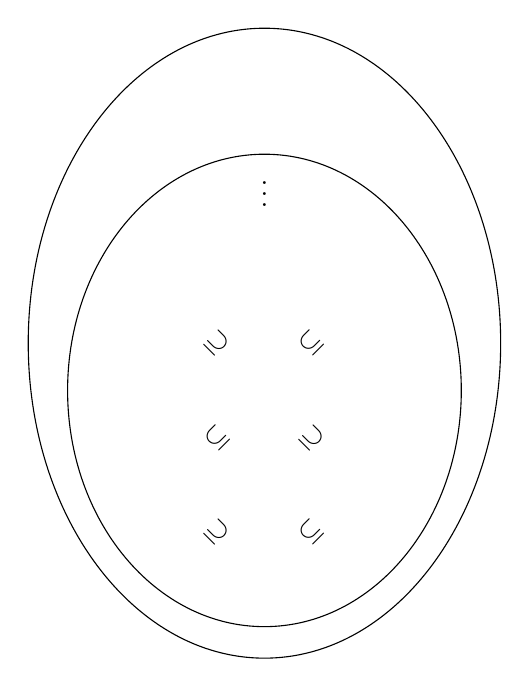
\begin{tikzpicture}[point/.style={draw,circle,inner sep=0cm,fill=black,minimum size=2pt}]
        \node (n1) at (0,0) {$\PClass$};
        \node (n2) at (1.2,1.2) {$\NPClass$};
        \node (n3) at (-1.2,1.2) {$\CONPClass$};
        \node () at (0,5) {$\vdots$};
        \node (n4) at (0,2.4) {$\PClass^{\NPClass}$};
        \node (n5) at (1.2,3.6) {$\NPClass^{\NPClass}$};
        \node (n6) at (-1.2,3.6) {$\CONPClass^{\NPClass}$};
        \path (n1) -- (n2) node [pos=0.5,sloped] {$\subseteq$};
        \path (n1) -- (n3) node [pos=0.5,sloped] {$\supseteq$};
        \path (n4) -- (n5) node [pos=0.5,sloped] {$\subseteq$};
        \path (n4) -- (n6) node [pos=0.5,sloped] {$\supseteq$};
        \path (n2) -- (n4) node [pos=0.5,sloped] {$\supseteq$};
        \path (n3) -- (n4) node [pos=0.5,sloped] {$\subseteq$};
        \draw (0,2.4) circle [x radius=2.5cm,y radius=3cm];
        \draw (0,3) circle [x radius=3cm,y radius=4cm];
        \node () at (0,6.25) {$\PSPACE$};
    \end{tikzpicture}
\end{document}
